\documentclass[11pt, a4paper]{article}

% --- Core Packages ---
\usepackage[utf8]{inputenc}
\usepackage[T1]{fontenc}
\usepackage{geometry}
\usepackage{amsmath, amssymb, amsfonts}
\usepackage{graphicx}
\usepackage{hyperref}
\usepackage{setspace}
\usepackage{titlesec}
\usepackage{cite}
\usepackage{tikz} % THIS DRAWS THE FIGURES
\usetikzlibrary{shapes,arrows,positioning,calc}

% --- Page Layout ---
\geometry{left=2.5cm, right=2.5cm, top=2.5cm, bottom=2.5cm}
\onehalfspacing

\title{\textbf{The Fragmentation Problem in the Sciences of Mind and Society: \\ A Minimal Unified Framework}}
\author{\textbf{[PRINCE T PHILIP]} \\ \texttt{github.com/psycho-prince/five-rule-framework}}
\date{\today}

\begin{document}

\maketitle

\begin{abstract}
\noindent This paper proposes a minimal unified framework consisting of five interacting principles: \textbf{Prediction}, \textbf{Feedback}, \textbf{Attention}, \textbf{Self-Modeling}, and \textbf{Social Coupling}. We provide a continuous mathematical path from neural computation to social organization.
\end{abstract}

\section{The Five-Rule Framework}

\subsection{Visualizing the Hierarchy (Figure 1)}
The following diagram establishes the continuity from neural mechanisms to societal organization.

\begin{figure}[ht]
\centering
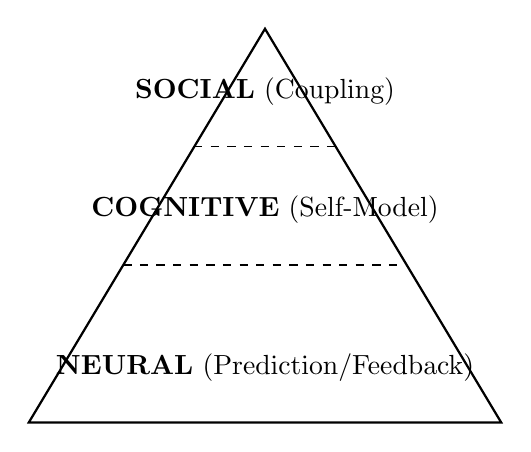
\begin{tikzpicture}[node distance=1.5cm, auto]
    % Draw the Pyramid
    \draw[thick] (0,0) -- (6,0) -- (3,5) -- cycle;
    \draw[dashed] (1.2,2) -- (4.8,2);
    \draw[dashed] (2.1,3.5) -- (3.9,3.5);
    
    % Labels
    \node at (3,0.7) {\textbf{NEURAL} (Prediction/Feedback)};
    \node at (3,2.7) {\textbf{COGNITIVE} (Self-Model)};
    \node at (3,4.2) {\textbf{SOCIAL} (Coupling)};
\end{tikzpicture}
\caption{Hierarchy of the Five-Rule Framework across scales.}
\label{fig:layered}
\end{figure}

\subsection{The Operational Loop (Figure 2)}
This represents the computational cycle of a single agent.

\begin{figure}[ht]
\centering
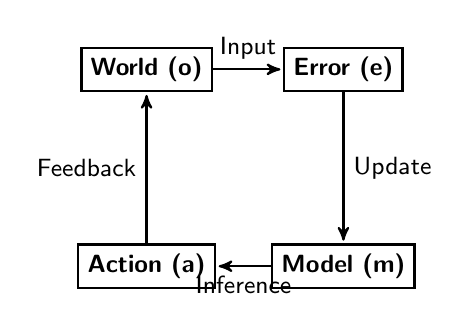
\begin{tikzpicture}[->,>=stealth',shorten >=1pt,auto,node distance=2.5cm,
  thick,main node/.style={rectangle,draw,font=\sffamily\small\bfseries}]

  \node[main node] (1) {World (o)};
  \node[main node] (2) [right of=1] {Error (e)};
  \node[main node] (3) [below of=2] {Model (m)};
  \node[main node] (4) [left of=3] {Action (a)};

  \path[every node/.style={font=\sffamily\small}]
    (1) edge node [above] {Input} (2)
    (2) edge node [right] {Update} (3)
    (3) edge node [below] {Inference} (4)
    (4) edge node [left] {Feedback} (1);
\end{tikzpicture}
\caption{The Feedback loop: Prediction error driving model updates and action.}
\label{fig:mathflow}
\end{figure}

\section{Formalisms and Conclusion}
(Include the Prediction, Feedback, and Attention equations here as previously drafted.)

\begin{thebibliography}{99}
\bibitem{friston2010} Friston, K. (2010). The free-energy principle: a unified brain theory? \textit{Nature Reviews Neuroscience}.
\end{thebibliography}

\end{document}

